\chapter{GROUP THEORY}

\section{INTRODUCTION TO GROUPS}

\subsection{BASIC AXIOMS}

\begin{definition}[Group]
	A group is an ordered pair $(G, \cdot)$ where $G$ is a set and $\cdot$ is a binary operation on $G$ such that
	\begin{itemize}
		\item There exists an element $e \in G$, namely identity, such that $ae = ea = e$ for each $a \in G$
		\item For each $a \in G$, there exists an element $a^{-1}$, namely inverse, such that $a a^{-1} = a^{-1} a = e$
		\item $\cdot$ is associative, that is, $(ab)c = a(bc)$ for all $a, b, c \in G$
	\end{itemize}
	A group $(G, \cdot)$ is said to be abelian if $\cdot$ is commutative, that is, $ab = ba$ for all $a, b \in G$
\end{definition}

\begin{definition}[Direct Product]
	If $(A, \star), (B, \diamond)$ are groups, the direct product $(A, \star) \times (B, \diamond)$ is a group of $A \times B$ under $\cdot$ defined as
	\[
	A \times B = \set{(a, b): a \in A, b \in B}
	\]
	\[
	(a_1, b_1) \cdot (a_2, b_2) = (a_1 \star a_2, b_1 \diamond b_2)
	\]
\end{definition}

\begin{proposition}[Basic Properties]
	If $G$ is a group under $\cdot$, then
	\begin{enumerate}
		\item The identity of $G$ is unique
		\item The inverse is unique for each $a \in G$
		\item $(a^{-1})^{-1} = a$ for each $a \in G$
		\item $(ab)^{-1} = b^{-1} a^{-1}$
	\end{enumerate}
\end{proposition}

\begin{proposition}[Cancellation Laws]
	Let $G$ be a group and $a, b \in G$. The two equations below have unique solutions
	\begin{itemize}
		\item $ax = b$
		\item $ya = b$
	\end{itemize}
	That is, $x = a^{-1} b$, $y = b a^{-1}$
\end{proposition}

\begin{definition}[Order of An Element]
	Let $G$ be a group and $x \in G$. Let $n$ be the smallest positive integer such that $x^n = 1$. $n$, denoted by $|x|$, is said to be the order of $x$. If there is no positive integer $n$ satisfying $x^n = 1$, the order of $x$ is said to be infinity.
\end{definition}

\subsection{DIHEDRAL GROUP}

\begin{definition}[$D_{2n}$ - Dihedral Group of Order $2n$]
	The symmetry group of a regular $n$-polygon. Let $r$ be the rotation clockwise about the origin through $2\pi/n$ radian and $s$ be the reflection about the line of symmetry through vertex $1$ and the origin. The following are true
	\begin{enumerate}
		\item $1, r, r^2, ..., r^{n-1}$ are distinct and $r^n = 1$, so $|r| = n$
		\item $|s| = 2$
		\item $D_{2n} = \set{1, r, r^2, ..., r^{n-1}, s, sr, sr^2, ..., sr^{n-1}}$, $|D_{2n}| = 2n$
		\item $rs = sr^{-1}$, more generally, $r^is - sr^{-i}$ for all $i \in \Z$
	\end{enumerate}
\end{definition}

\subsubsection{Generators and Relations}

\begin{definition}[Generators and Relations]
	A subset $S$ of a group $G$ is said to be the set of generators of $G$ if every element of $G$ can be written as a finite product of elements of $S$, denoted by $G = \inner{S}$.
	Furthermore, the equations that elements of $S$ satisfy are said to be relations, denoted by $R_1, R_2, ..., R_m$. We write
	\[
	G = \inner{S | R_1, R_2, ..., R_m}
	\]
	The dihedral group $D_{2n}$ can be written as 
	\[
	D_{2n} = \inner{r, s | r^n = s^2 = 1, rs = sr^{-1}}
	\]
\end{definition}

\subsection{SYMMETRIC GROUP}

\begin{definition}[Symmetric Group]
	Let $\Omega$ be a nonempty set and $S_\Omega$ be the set of all bijections from $\Omega$ onto itself (i.e the set of all permutations of $\Omega$). $S_\Omega$ is a group under function composition $\circ$, namely the symmetric group on $\Omega$.
\end{definition} 

\subsection{MATRIX GROUP}

\begin{definition}[Field]
	A field is a set $F$ equipped with two binary operations $+$ and $\cdot$ such that $(F, +)$ is an abelian group with its (additive) identity $0$ and $(F \setminus \set{0}, \cdot)$ is an abelian group with its (multiplicative) identity $1$ and the distributive law holds
	\[
	a(b+c) = ab + ac \text{ for all $a, b, c \in F$}
	\]
	Let $F^{\times}$ denotes $F \setminus \set{0}$
\end{definition}

\begin{definition}[General Linear Group]
	Let $GL_{n}(F)$ be the set of all $n \times n$ matrices whose entries come from $F$ and the determinant is nonzero. Then $GL_{n}(F)$ is a group under matrix multiplication, namely the general linear group of degree $n$
\end{definition}

\subsection{QUATERNION GROUP}

\begin{definition}[Quaternion Group]
	The quaternion group $Q_8$ is defined by
	\[
	Q_8 = \set{1, -1, i, -i, j, -j, k, -k}
	\]
	where the operation is defined as follows
	\begin{itemize}
		\item $1a = a1 = a$ for all $a \in Q_8$
		\item $(-1)(-1) = 1$, $(-1)a = a(-1) = -a$ for all $a \in Q_8$
		\item $ii = jj = kk = -1$
		\item $ij = k$, $ji = -k$
		\item $jk = i$, $kj = -i$
		\item $ki = j$, $ik = -j$
	\end{itemize}
\end{definition}

\subsection{HOMOMORPHISM AND ISOMORPHISM}

\begin{definition}[Homomorphism]
	Let $(G, \star)$ and $(H, \diamond)$ be groups. A map $\phi: G \to H$ is said to be a homomorphism if
	\[
	\phi(x \star y) = \phi(x) \diamond \phi(y) \text{ for all $x, y \in G$}
	\]
\end{definition}

\begin{definition}[Isomorphism]
	Let $(G, \star)$ and $(H, \diamond)$ be groups. A map $\phi: G \to H$ is said to be an isomorphism if $\phi$ is a homomorphism that is also a bijection.
	$G$ and $H$ are said to be isomorphic or of the same isomorphism type, denoted by $G \cong H$
\end{definition}

\subsection{GROUP ACTION}
\begin{definition}[Group Action]
	Let $G$ be a group and $A$ be a set. A map $\cdot: G \times A \to A$ (written in infix notation as $g \cdot a$ for $g \in G$ and $a \in A$) is said to be a group action of $G$ on $A$ if
	\begin{enumerate}
		\item $1 a = a$ for all $a \in A$
		\item $g_1 \cdot (g_2 \cdot a) = (g_1 g_2) \cdot a$ for all $g_1, g_2 \in G$ and $a \in A$
	\end{enumerate}
\end{definition}

\begin{definition}[Permutation Representation of Group Action]
	Let $\cdot$ be a group action of $G$ on $A$. For each $g \in G$, let $\sigma_g: A \times A$ be a permutation on $A$ such that $\sigma_g(a) = g \cdot a$ \footnote{this operation is well-defined}. Let $\phi: G \to S_A$ be defined as $\phi(g) = \sigma_g$. Then, $\phi$ is a homomorphism from $G$ to $S_A$, and it is said to be the permutation representation associated with $\cdot$.
\end{definition}

\section{SUBGROUPS}

\subsection{DEFINITION}

\begin{definition}[Subgroup]
	A subset $H$ of a group $G$ is said to be a subgroup if it is a group under the same operation, denoted by $H \leq G$.
\end{definition}

\begin{proposition}[Subgroup Criterion]
	A subset $H$ of a group $G$ is a subgroup if and only if
	\begin{enumerate}
		\item $H \neq \emptyset$
		\item $xy^{-1} \in H$ for all $x, y \in H$ 
	\end{enumerate}
	Furthermore, if $H$ is finite, it suffices to check that $H$ is nonempty and closed under multiplication.
\end{proposition}


\subsection{CENTRALIZER AND NORMALIZER, STABILIZER AND KERNEL}

\begin{definition}[Centralizer, Center]
	Given a group $G$ and a nonempty subset $A$ of $G$. Define 
	\[
	C_G(A) = \set{g \in G: \forall a \in A, gag^{-1} = a }
	\]
	Then, $C_G(A)$ is said to be the centralizer of $A$ in $G$. Furthermore, $C_G(A)$ is a subgroup of $G$.
	$Z(G) = C_G(G)$ is said to be the center of $G$.
\end{definition}

\begin{definition}[Normalizer]
	Given a group $G$ and a nonempty subset $A$ of $G$. Let
	\[
	N_G(A) = \set{g \in G: gAg^{-1} = A}
	\]
	where $gAg^{-1} = \set{gag^{-1}: a \in A}$. Then, the centralizer can be written as
	\[
	C_G(A) = \bigcap_{a \in A} N_G(\set{a})
	\]
\end{definition}

\subsubsection{Stabilizers and Kernels of Group Actions}

\begin{definition}[Stabilizer and Kernel]
	Let $\cdot$ be a group action of $G$ on $S$ and $s \in S$, define
	\[
	G_s = \set{g \in G: g \cdot s = s}
	\]
	Then, $G_s$ is said to be the stabilizer of $s$ in $G$. Furthermore, $G_s$ is a subgroup of $G$.
	Define the kernel of an action as 
	\[
	\set{g \in G: \forall s \in S, g \cdot s = s}
	\]
\end{definition}

\subsection{CYCLIC GROUPS AND CYCLIC SUBGROUPS}

\begin{definition}[Cyclic Group]
	A group $H$ is said to be cyclic if it can be generated by a single element, i.e. $H = \inner{x}$
\end{definition}

\begin{proposition}
	If $H = \inner{x}$, then $|H| = |x|$
\end{proposition}

\begin{proposition}
	Let $G$ be an arbitrary group and $x \in G$ and let $m, n \in \Z$. If $x^n = x^m = 1$, then $x^d = 1$ where $d = \gcd(m, n)$
\end{proposition}

\begin{theorem}
	Any two cyclic groups of the same order are isomorphic. Hence, the cyclic group of order $n$, $n \in \Z$, is denoted by $Z_n$
\end{theorem}

\begin{proposition}
	Let $G$ be a group, $x \in G$, and $a \in \Z \setminus \set{0}$
	\begin{enumerate}
		\item If $|x| = \infty$, then $|x^a| = \infty$
		\item If $|x| = n < \infty$, then $|x^a| = \frac{n}{\gcd(n, a)}$
	\end{enumerate}
\end{proposition}

\begin{proposition}
	Let $H = \inner{x}$
	\begin{enumerate}
		\item If $|x| = \infty$, then $H = \inner{x^a}$ if and only if $a = \pm 1$
		\item If $|x| = n < \infty$, then $H = \inner{x^a}$ if and only if $\gcd(a, n) = 1$
	\end{enumerate}
\end{proposition}

\begin{theorem}
	Let $H = \inner{x}$,
	\begin{enumerate}
		\item Every subgroup of $H$ is cyclic
		\item If $|H| = \infty$, then for any distinct positive integers $a, b$, $\inner{x^a} \neq \inner{x^b}$, for any integer $m$, $\inner{x^m} = \inner{x^{|m|}}$
		\item If $|H| = n < \infty$, for each positive integer $a$ dividing $n$, there is a unique subgroup of $H$ of order $a$ that is $\inner{x^d}$ where $d = \frac{n}{a}$. Furthermore, for every integer $m$, $\inner{x^m} = \inner{x^{(n, m)}}$, that is, there is a one-to-one correspondence between subgroups of $H$ and positive divisors of $n$
	\end{enumerate}
\end{theorem}

\subsection{SUBGROUPS GENERATED BY SUBSETS OF A GROUP}

\begin{proposition}
	If $\mathcal{A}$ is a nonempty collection of subgroups of $G$, the $K = \bigcap_{A \in \mathcal{A}} A$ is also a group of $G$
\end{proposition}

\begin{definition}[Subgroup Generated by a Subset]
	Let $A$ be a subset of group $G$, define
	\[
	\inner{A} = \bigcap_{A \subseteq H, H \leq G} H
	\]
	Then, $\inner{A}$ is said to be the subgroup generated by $A$
\end{definition}

\begin{proposition}
	Define the following
	\[
	\overline{A} = \set{ a_1^{\epsilon_1} a_2^{\epsilon_2} ... a_n^{\epsilon_n}: n \in \N, a_i \in A, \epsilon_i \in \Z}
	\]
	Then, $\overline{A} = \inner{A}$
\end{proposition}

\subsection{THE LATTICE OF SUBGROUPS OF A GROUP}

\section{QUOTIENT GROUPS AND HOMOMORPHISMS}

\subsection{DEFINITION}

\begin{definition}[Kernel of a Homomorphism]
	Let $\phi: G \to H$ be a homomorphism, define
	\[
	\ker \phi = \set{g \in G: \phi(g) = 1}
	\]
	Then, $\ker \phi$ is said to be the kernel of $\phi$.
\end{definition}

\begin{proposition}
	Let $\phi: G \to H$ be a homomorphism, then
	\begin{enumerate}
		\item $\phi(1_G) = 1_H$ where $1_G$ and $1_H$ are the identities of $G$ and $H$ respectively
		\item $\phi(g^n) = \phi(g)^n$ for all $g \in G, n \in \Z$
		\item $\ker \phi$ is a subgroup of $G$
		\item $\im G$, the image of $G$ under $\phi$ is a subgroup of $H$
	\end{enumerate}
\end{proposition}

\begin{definition}[Quotient Group]
	Let $\phi: G \to H$ be a homomorphism with kernel $K$. The quotient group, denoted by $G/K$, is the group whose elements are the fibers of $\phi$ over the elements of $\im G \subseteq H$ with group operation $\cdot$ defined as
	\[
	\phi^{-1}(a) \cdot \phi^{-1}(b) = \phi^{-1}(ab)
	\]
	for all $a, b \in \im G$
\end{definition}

\begin{proposition}
	Let $\phi: G \to H$ be a homomorphism with kernel $K$. Let $X \in G/K$ be the fiber if $\phi$ over $a$, that is, $X = \phi^{-1}(a)$. Then,
	\begin{enumerate}
		\item For any $u \in X$, $uX = \set{uk: k \in K}$
		\item For any $u \in X$, $Xu = \set{ku: k \in K}$
	\end{enumerate}
\end{proposition}

\begin{definition}[Coset]
	Let $G$ be a group, for any $N \leq G$ and any $g \in G$, let
	\[
	gN = \set{gn: n \in N} \text{ and } Ng = \set{ng: n \in N}
	\]
	Then, $gN$ and $Ng$ are said to be the left coset and the right coset of $N$ in $G$.
\end{definition}

\begin{theorem}
	Let $G$ be a group and $K$ be the kernel of some homomorphism from $G$. Then the set whose elements are the left cosets of $K$ in $G$ with the operation defined as
	\[
	uK \cdot vK = (uv)K
	\]
	for $u, v \in G$ forms the quotient group $G/K$
\end{theorem}

\begin{proposition}
	Let $N$ be any subgroup of $G$, then the set of left cosets of $N$ in $G$ partitions $G$. Furthermore, for all $u, v \in G$, $uN = vN$ if and only if $uv^{-1} \in N$
\end{proposition}


\begin{proposition}
	Let $G$ be a group and let $N$ be a subgroup of $G$
	\begin{enumerate}
		\item The operation on the left cosets of $N$ in $G$ described by
		\[
		uN \cdot vN = (uv) N
		\]
		is well-defined if and only $gng^{-1} \in N$ for all $g \in G$ and all $n \in N$
		\item If the above operation is well-defined, then the set of left cosets of $N$ in $G$ forms a group. In particular, the identity of this group is $N$ and the inverse of $gN$ is $g^{-1}N$
	\end{enumerate}
\end{proposition}

\begin{definition}[Conjugate, Normalize, Normal Subgroup]
	The element $gng^{-1}$ is called the conjugate of $n \in N$ by $g$. The set $gNg^{-1} = \set{gng^{-1}: n \in N}$ is said to be the conjugate of $N$ by $g$. The element $g$ is said to normalize $N$ if $gNg^{-1} = N$, i.e $g \in N_G(N)$. A subgroup $N$ of $G$ is said to be normal, denoted by $N \trianglelefteq G$, if every element of $G$ normalizes $N$, i.e. $N_G(N) = G$
\end{definition}

\begin{theorem}
	Let $N$ be a subgroup of $G$. The following are equivalent:
	\begin{enumerate}
		\item $N \trianglelefteq G$
		\item $N_G(N) = G$
		\item $gN = Ng$ for all $g \in G$
		\item the set of left cosets form a group under the operation $uN \cdot vN = (uv) N$
	\end{enumerate}
\end{theorem}

\begin{proposition}
	A subgroup $N$ of $G$ is normal if and only if it is the kernel of some homomorphism
\end{proposition}

\begin{definition}[Natural Projection, Complete Preimage]
	Let $N \trianglelefteq G$. The homomorphism $\pi: G \to G/N$ defined by $\phi(g) = gN$ is said to be the natural projection of $G$ onto $G/N$. If $\overline{H} \leq G/N$ is a subgroup of $G/N$, the complete preimage of $\overline{H}$ in $G$ is $\pi^{-1}(\overline{H})$
\end{definition}

\subsection{MORE ON COSETS AND LAGRANGE THEOREM}

\begin{theorem}[Lagrange Theorem]
	Let $H$ be a subgroup of a finite group $G$, then the order of $H$ divides $G$ and the number of left cosets of $H$ in $G$ is $\frac{|G|}{|H|}$
\end{theorem}

\begin{definition}[Index of a Subgroup]
	Let $H \leq G$, the number of left cosets of $H$ in $G$ is said to be the index of $H$ in $G$, denoted by $|G:H|$
\end{definition}

\begin{corollary}
	If $G$ is a finite group and $x \in G$, the order of $x$ divides the order of $G$. In particular, $x^{|G|} = 1$ for all $x \in G$
\end{corollary}

\begin{corollary}
	If $G$ is a group of prime order $p$, then $G$ is cyclic, hence $G \cong Z_p$
\end{corollary}

\begin{theorem}[Cauchy Theorem]
	If $G$ is a finite group and $p$ is a prime dividing $|G|$, then $G$ has an element of order $p$
\end{theorem}

\begin{theorem}[Sylow Theorem]
	If $G$ is a finite group of order $p^\alpha m$ where $p$ is a prime and $p$ does not divide $m$, then $G$ has a subgroup of order $p^\alpha$
\end{theorem}

\begin{definition}
	Let $H, K$ be subgroups of a group, define
	\[
	HK = \set{hk: h \in H, k \in K} = \bigcup_{h \in H} hK
	\]
\end{definition}

\begin{proposition}
	If $H$ and $K$ are finite subgroups of a group then
	\[
	|HK| = \frac{|H||K|}{|H \cap K|}
	\]
\end{proposition}

\begin{proposition}
	If $H$ and $K$ are finite subgroups of a group then, $HK$ is a subgroup if and only if $HK = KH$
\end{proposition}

\begin{corollary}
	If $H$ and $K$ are subgroups of $G$ and $H \leq N_G(K)$, then $HK$ is a subgroup of $G$. In particular, if $K \trianglelefteq G$, the $HK \leq G$ for any $H \leq G$
\end{corollary}

\begin{definition}[Normalize, Centralize]
	$A$ is said to normalize $K$ (or centralize $K$) if $A \subseteq N_G(K)$ (or $A \subseteq C_G(K)$)
\end{definition}

\subsection{THE ISOMORPHISM THEOREMS}

\begin{theorem}[the first isomorphism theorem]
	If $\phi: G \to H$ is a homomorphism, then $\ker \phi \trianglelefteq G$ and $G / \ker \phi \cong \im \phi$
	
	\note{The map $\phi: (x, y) \to (x, 0)$ on $G = \R^2$ has the kernel $\ker \phi = \set{(0, y): y \in \R}$ which is the line parallel to the $y$-coordinate and intersects $x$-coordinate at $x=0$. $G/\ker \phi$ is the set of all lines parallel to the $y$-coordinate which is isomorphic to the image $\im \phi = \set{(x, 0): x \in \R}$}
	
	
\end{theorem}

\begin{corollary}
	If $\phi: G \to H$ is a homomorphism. Then,
	\begin{enumerate}
		\item $\phi$ is injective if and only if $\ker \phi = \set{1}$
		\item $|G : \ker \phi| = |\im G|$
	\end{enumerate}
\end{corollary}

\begin{theorem}[the second isomorphism theorem, the diamond isomorphism theorem]
	Let $A, B$ be subgroups of $G$ with $A$ normalizes $B$, then $AB$ is a subgroup of $G$, and 
	$$
	\frac{AB}{B} \cong \frac{A}{A \cap B}
	$$
	
	where subgroups being normal as necessary
	
	\begin{center}
		\begin{tikzcd}
			& G                                          &                          \\
			& AB \arrow[u]                               &                          \\
			A \arrow[ru] &                                            & B \arrow[lu, Rightarrow] \\
			& A \cap B \arrow[ru] \arrow[lu, Rightarrow] &                          \\
			& 1 \arrow[u]                                &                         
		\end{tikzcd}
	\end{center}
	
	Additionally, $A$ need not to be normal in $AB$, we still have $|AB : A| = |B : A \cap B|$
	
	\note{$A = \set{(x, y, 0): x, y \in \R}$ and $B = \set{(0, y, z): y, x \in \R}$ are subgroups of $G = \R^3$ with $AB = G = \set{(x, y, z): x, y, z \in \R}$, $A \cap B = \set{(0, y, 0): y \in \R}$. $AB / B$ is the set of all planes orthogonal to the $x$-coordinate. $A / A \cap B$ is the set of all lines on $(x, y)$-plane that is orthogonal to the $x$-coordinate. Both are isomorphic to the $x$-coordinate}
\end{theorem}


\begin{figure}
	\centering
	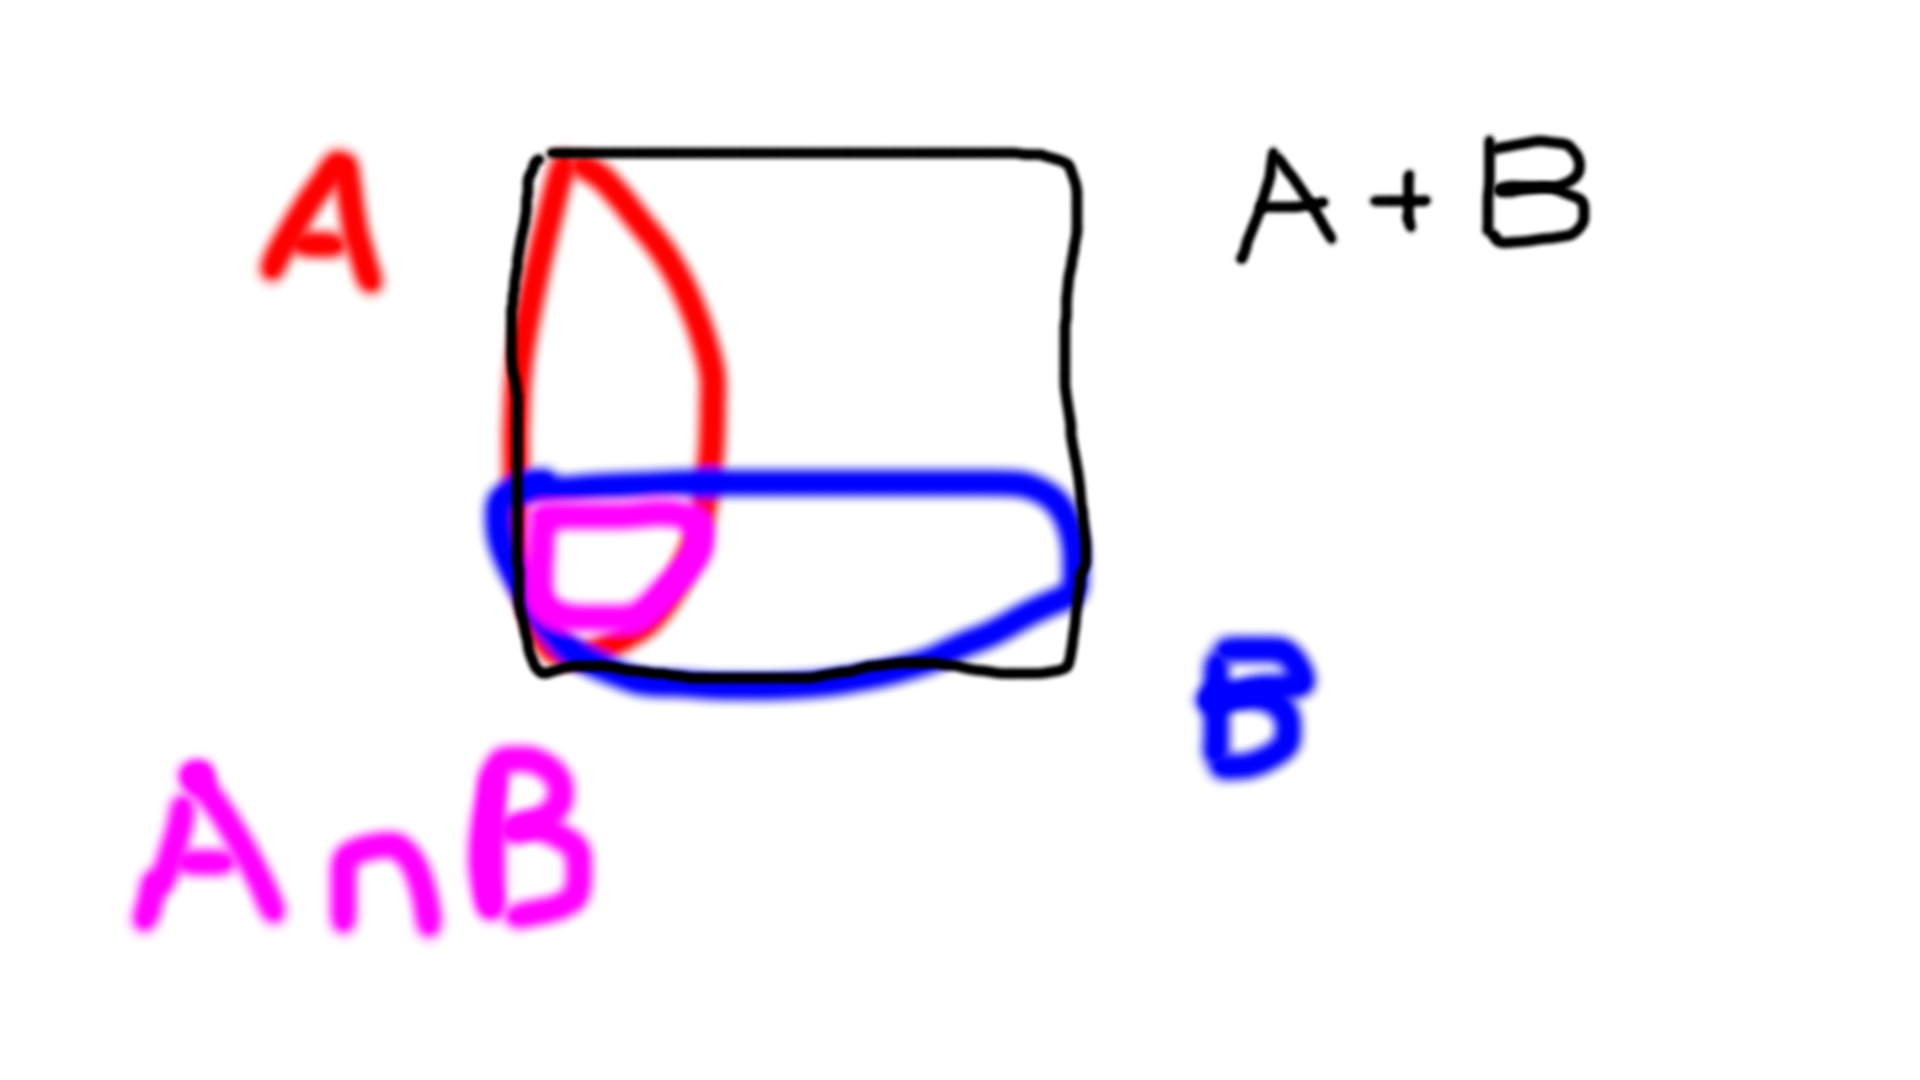
\includegraphics[width=0.8\textwidth]{assets/second_isomorphism.png}
	\caption{second isomorphsim theorem}
\end{figure}


\begin{theorem}[The Third Isomorphism Theorem]
	Let $H, K$ be normal subgroups of $G$ with $H \leq K$. Then
	\[
	\frac{G/H}{K/H} \cong \frac{G}{K}
	\]
	where subgroups being normal as necessary
	
	\note{$G = \set{(x, y, z): x, y, z \in \R} = \R^3$, $K = \set{(x, y, 0): x, y \in \R}$, then $G/K$ is the set of all planes orthogonal to the $z$-coordinate that is isomorphic to $z$-coordinate. $H = \set{(x, 0, 0): x \in \R}$, $G/H$ is the set of all lines paralllel to the $x$-coordinate that can be identified with the $(y, z)$-plane, $K/H$ is the set of all lines on $(x, y)$-plane parallel to the $x$-coordinate that can be identified with the $y$-coordinate, then $(G/H)/(K/H)$ can be identified with the the $z$-coordinate}
\end{theorem}

\begin{theorem}[the forth isomorphism theorem, the lattice isomorphism theorem]
	Let $N$ be a normal subgroup of $G$, then there is a one-to-one correspondence between the set of subgroups of $G$ containing $N$ and the set of subgroups of $\overline{G} = G/N$. Let $A$ be a subgroup of $G$ containing $N$, then $\overline{A} = A/I$ is the corresponding subgroup of $\overline{G} = G/N$. The bijection has the following properties
	\begin{enumerate}
		\item $A \leq B$ if and only if $\overline{A} \leq \overline{B}$
		\item if $A \leq B$, then $|B:A| = |\overline{B}:\overline{A}|$
		\item $\overline{\inner{A, B}} = \inner{\overline{A}, \overline{B}}$
		\item $\overline{A \cap B} = \overline{A} \cap \overline{B}$
		\item $A \trianglelefteq G$ if and only if $\overline{A} \trianglelefteq \overline{G}$
	\end{enumerate}
	
	\note{
		In the $3$-dimensional Cartesian coordinates $G = \set{(x, y, z): x, y, z \in \R}$, the $x$-coordinate $N = \set{(x, 0, 0): x \in \R}$ is a normal subgroup of $G$. $G/N$ is the collection of lines parallel to the $x$-coordinate $N$, that is isomorphic to the $(y,z)$-plane $\set{(0, y, z): y, z \in \R}$
	}
	
	\note{
		On one hand, the set of subgroups of $G$ containing $N$ consists of $N$, $G$, and all planes containing $N$.	Each plane containing $N$ corresponds to a nonzero point on the $(y,z)$-plane
	}
	
	\note{
		On the other hand, the set of subgroups of $G/N$ consists of $\set{0}$, the whole space, and all lines going through $0$ on the $(y,z)$-plane
	}
\end{theorem}

\subsection{COMPOSITION SERIES AND THE HÖLDER PROGRAM}

\begin{proposition}[Cauchy Theorem for abelian groups]
	If $G$ is a finite abelian group and $p$ is a prime dividing $|G|$, then $G$ contains an element of order $p$
\end{proposition}

\begin{definition}[Simple Group]
	A group $G$ is said to be simple if $|G| > 1$ and the only normal subgroups of $G$ are $1$ and $G$
\end{definition}

\begin{definition}[Composition Series]
	A sequence of groups
	\[
	1 = N_0 \leq N_1 \leq ... \leq N_k = G
	\]
	is said to be a composition series if $N_{i-1} \trianglelefteq N_i$ and $N_i / N_{i-1}$ is simple for all $1 \leq i \leq k$. Moreover, the quotient groups $N_i / N_{i-1}$ are said to be the composition factors of $G$
\end{definition}

\begin{theorem}[Jordan-Hölder]
	Let $G$ be a nontrivial finite group. Then
	\begin{enumerate}
		\item $G$ has a composition series
		\item The composition factors in a composition series are unique. That is, if $1 \trianglelefteq N_0 \trianglelefteq ... \trianglelefteq N_r = G$ and $1 \trianglelefteq M_0 \trianglelefteq ... \trianglelefteq M_s = G$, then $r = s$ and there is a permutation $\pi$ such that
		\[
		M_{\pi(i)} / M_{\pi(i)-1} \cong N_{i} / N_{i-1}
		\]
		for all $1 \leq i \leq r$
	\end{enumerate}
\end{theorem}

\begin{theorem}[Part 1 of the Hölder Program]
	There is a list consisting of 18 families of simple groups and 26 simple groups not belong to these families (the sporadic simple groups) such that every finite simple group is isomorphic to one of the groups in this list
\end{theorem}

\begin{theorem}[Feit-Thompson]
	If $G$ is a simple group of odd order, then $G \cong Z_p$ for some prime $p$
\end{theorem}

\begin{definition}[Solvable Group]
	A group $G$ is said to be solvable if there is a chain of subgroups 
	\[
	1 \trianglelefteq G_0 \trianglelefteq ... \trianglelefteq G_s = G
	\]
	such that $G_i / G_{i-1}$ is abelian for all $1 \leq i \leq s$
\end{definition}

\begin{theorem}
	The finite group $G$ is solvable if and only for every divisor $n$ of $|G|$ such that $\tuple{n, \frac{|G|}{n}} = 1$, $G$ has a subgroup of order $n$
\end{theorem}


\subsection{TRANSPOSITION AND THE ALTERNATING GROUP}

\subsubsection{Transpositions and Generation of $S_n$}

\begin{definition}[Transposition]
	A $2$-cycle is said to be a transposition
\end{definition}

\begin{proposition}
	Every element of $S_n$ can be written as a product of transpositions
\end{proposition}

\subsubsection{The Alternating Group}

\begin{definition}[Parity of Permutation]
	For any $\sigma \in S_n$, define the polynomial $\Delta$
	\[
	\Delta = \prod_{1 \leq i < j \leq n} (x_i - x_j)
	\]
	Let $\sigma$ act on $\Delta$ by
	\[
	\sigma(\Delta) = \prod_{1 \leq i < j \leq n} (x_{\sigma(i)} - x_{\sigma(j)})
	\]
	Define the sign of $\sigma$ as
	\[
	\epsilon(\sigma) = \begin{cases}
		+1 \;\;\;\text{if $\sigma(\Delta) = +\Delta$} \\
		-1 \;\;\;\text{if $\sigma(\Delta) = -\Delta$}
	\end{cases}
	\]
	$\sigma$ is said to be an even permutation if $\epsilon(\sigma) = +1$, and odd permutation if $\epsilon(\sigma) = -1$
\end{definition}

\begin{proposition}
	The map $\epsilon: S_n \to \set{-1, +1}^{\times}$ is a homomorphism
\end{proposition}

\begin{proposition}
	Transpositions are all odd permutations and $\epsilon$ is a surjective homomorphism
\end{proposition}

\begin{definition}[Alternating Group]
	The kernel of homomorphism $\epsilon$ is said to be the alternating group of degree $n$, denoted by $A_n$
\end{definition}

\begin{proposition}
	The permutation $\sigma$ is odd if and only the number of cycles of even length in its cycle decomposition is odd
\end{proposition}

\section{GROUP ACTIONS}

\subsection{GROUP ACTIONS AND PERMUTATION REPRESENTATIONS}

\begin{definition}
	Some definitions related to group actions
	\begin{enumerate}
		\item The set of elements in $G$ that act trivially on $A$, namely $\set{g \in G: \forall a \in A, g \cdot a = a}$, is said to be the kernel of the action
		\item For each $a \in A$, the set of elements in $G$ that fix $a$, namely $G_a = \set{g \in G: g \cdot a = a}$, is said to be the stabilizer of $a$
		\item An action is said to be faithful if its kernel is the identity
	\end{enumerate}
\end{definition}

\begin{proposition}
	Let group $G$ act on a nonempty set $A$, there is a one-to-one correspondence between the actions of $G$ on $A$ and the homomorphisms from $G$ into $S_A$
\end{proposition}

\begin{definition}[Permutation Representation]
	For any group $G$ and nonempty set $A$, any homomorphism from $G$ into $S_A$ is said to be a permutation representation of $G$
\end{definition}

\begin{proposition}[Orbit-Stabilizer Theorem]
	Let group $G$ act on a nonempty set $A$. The relation defined by
	\[
	a \sim b \text{ if and only if for some $g \in G$, } b = g \cdot a
	\]
	is an equivalence relation. Furthermore, for each $a \in A$, let $C_a$ be the equivalence class containing $a$. impose the group structure on $C_a$ with $\star: C_a \times C_a \to C_a$ defined by
	\[
	x \star y = (g_x g_y) \cdot a
	\]
	where $x = g_x \cdot a$, $y = g_y \cdot a$. Then, the map $g \mapsto g \cdot a$ is a surjective homomorphism from $G$ to $C_a$. Consequently, $|C_a| = |G / G_a|$ where $G_a$ is the stabilizer of $a$
\end{proposition}

\begin{definition}[Orbit]
	Let group $G$ act on a nonempty set $A$
	\begin{enumerate}
		\item The equivalence class $C_a = \set{g \cdot a: g \in G}$ is said to be the orbit of $G$ containing $a$
		\item The action of $G$ on $a$ is said to be transitive if there is only one orbit
	\end{enumerate}
\end{definition}

\subsubsection{Cycle Decompositions}

\subsection{GROUPS ACTING ON THEMSELVES BY LEFT MULTIPLICATION - CAYLEY THEOREM}

\begin{theorem}
	Let $H$ be a subgroup of $G$ and $G$ act by left multiplication on the set $A$ of left cosets of $H$, i.e. the action is defined by $g \cdot xH = gxH$. Let $\pi_H: G \to S_A$ be the associated permutation representation afforded by this action. Then
	\begin{enumerate}
		\item $G$ acts transitively on $A$
		\item The stabilizer in $G$ of the point $1H \in A$ is the subgroup $H$
		\item $\ker \pi_H = \bigcap_{x \in G} xHx^{-1}$ and it is the largest normal subgroup of $G$ contained in $H$
	\end{enumerate}
\end{theorem}

\begin{corollary}[Cayley Theorem]
	Every group is isomorphic to a subgroup of some symmetric group. If $|G| = n$, then $G$ is isomorphic to a subgroup of $S_n$
	
	\note{TODO - add yoneda lemma here}
\end{corollary}

\begin{corollary}
	If $G$ is a finite group of order $n$ and $p$ is the smallest prime dividing $|G|$, then any subgroup of of index $p$ is normal
\end{corollary}

\subsection{GROUPS ACTING ON THEMSELVES BY CONJUGATION - THE CLASS EQUATION}

\begin{definition}[Conjugate, Conjugacy Class]
	Two elements $a, b \in G$ are said to be conjugate in $G$ if there exists $g \in G$ such that $b = gag^{-1}$, i.e. $a, b$ in the same orbit of $G$ acting on itself by conjugation. The orbits of $G$ acting on itself by conjugation is said to be the conjugacy classes of $G$
\end{definition}

\begin{definition}[Conjugate]
	Two subsets $S, T \subseteq G$ are said to be conjugate in $G$ if there exists $g \in G$ such that $T = gSg^{-1}$, i.e. $S, T$ in the same orbit of $G$ acting on its subsets by conjugation
\end{definition}

\begin{proposition}
	The number of conjugates of a subset $S$ in a group $G$ is the index of the normalizer of $S$, $|G : N_G(S)|$, i.e. the stabilizer of $G$ acting on its subsets by conjugation. In particular, the number of conjugates of an element $s$ of $G$ is the index of the centralizer of $s$, $|G : C_G(s)|$
\end{proposition}

\begin{theorem}[The Class Equation]
	Let $G$ be a finite group and $g_1, g_2, ..., g_r$ be representatives of the distinct conjugacy classes of $G$ not contained in the center $Z(G)$. Then
	\[
	|G| = |Z(G)| + \sum_{i=1}^r |G : C_G(g_i)|
	\]
	Each element $z \in Z(G)$ can be considered as a singleton conjugacy class.
\end{theorem}

\begin{theorem}
	If $p$ is a prime and $P$ is a group of prime power order $p^\alpha$ for some $\alpha \geq 1$, then $P$ has a nontrivial center $Z(P) \neq 1$
\end{theorem}

\begin{corollary}
	If $|P| = p^2$ for some prime $p$, then $P$ is abelian. More precisely, $P$ is isomorphic to either $Z_{p^2}$ or $Z_p \times Z_p$
\end{corollary}

\subsubsection{Conjugacy in $S_n$}

\begin{proposition}
	Let $\sigma, \tau \in S_n$ and suppose $\sigma$ has the cycle decomposition
	\[
	(a_1 a_2 ... a_{k_1}) (b_1 b_2 ... b_{k_2}) ...
	\]
	Then $\tau \sigma \tau^{-1}$ has the cycle decomposition
	\[
	(\tau(a_1) \tau(a_2) ... \tau(a_{k_1})) (\tau(b_1) \tau(b_2) ... \tau(b_{k_2})) ...
	\]
\end{proposition}

\begin{definition}[Cycle Type]
	If $\sigma \in S_n$ is the product of disjoint cycles of length $n_1, n_2, ..., n_r$ with $n_1 \leq n_2 \leq ... \leq n_r$ (including $1$-cycles) then the sequence $n_1, n_2, ..., n_r$ is said to be the cycle type of $\sigma$
\end{definition}

\begin{definition}[Partition of a Positive Integer]
	Given $n \in \N$, a sequence of nondecreasing positive integers whose sum is $n$ is said to be a partition of $n$
\end{definition}

\begin{proposition}
	Two elements of $S_n$ are conjugate in $S_n$ if and only if they have the same cycle type. The number of conjugacy classes of $S_n$ is the number of partitions of $n$
\end{proposition}

\begin{proposition}
	Any normal subgroup of $G$ is a union of conjugacy classes of $G$
\end{proposition}

\begin{theorem}
	$A_5$ is a simple group
\end{theorem}

\subsubsection{Right Group Actions}

\subsection{AUTOMORPHISMS}

\begin{definition}[Automorphism]
	An isomorphism from a group $G$ onto itself is said to be an automorphism of $G$. The set of all automorphisms of $G$ is denoted by $\Aut(G) \subseteq S_G$
\end{definition}

\begin{proposition}
	Let $H$ be a normal subgroup of $G$. Then $G$ acts by conjugation on $H$ as automorphisms of $H$. For each $g \in G$, conjugation by $g$ is an automorphism of $H$. The permutation representation afforded by this action is a homomorphism from $G$ into $\Aut(H)$ with kernel $C_G(H)$. In particular, $G / C_G(H)$ is isomorphic to a subgroup of $\Aut(H)$
\end{proposition}

\begin{corollary}
	If $K$ is any subgroup of $G$ and $g \in G$, then $K \cong gKg^{-1}$. Conjugate elements and conjugate subgroups have the same order.
\end{corollary}

\begin{corollary}
	For any subgroup $H$ of $G$, the quotient group $N_G(H) / C_G(H)$ is isomorphic to a subgroup of $\Aut(H)$. In particular, $G/Z(G)$ is isomorphic to a subgroup of $\Aut(H)$
\end{corollary}

\begin{definition}[Inner Automorphism]
	Let $G$ be a group and $g \in G$. Conjugation by $g$ is said to be an inner automorphism of $G$ and the subgroup of $\Aut(G)$ consisting of all inner automorphisms is denoted by $\inn(G)$
\end{definition}

\begin{definition}[Characteristic]
	A subgroup $H$ of $G$ is said to be characteristic in $G$, denoted by $H \Char G$, if every automorphism of $G$ maps $H$ into itself, i.e. for all $\sigma \in \Aut(G)$, $\sigma(H) = H$
\end{definition}

\begin{proposition}
	Some results concerning characteristic subgroups
	\begin{enumerate}
		\item Characteristic subgroups are normal
		\item if $H$ is the unique subgroup of $G$ of a given order, then $H$ is characteristic in $G$
		\item if $K \Char H$ and $H \trianglelefteq G$, then $K \trianglelefteq G$
	\end{enumerate}
\end{proposition}

\begin{proposition}
	The automorphism group of the cyclic group of order $n$ is isomorphic to $(\Z / n\Z)^\times$, an abelian group of order $\phi(n)$ where $\phi$ is the Euler function.
\end{proposition}

\begin{proposition}
	Some results on automorphism groups
	\begin{enumerate}
		\item If $p$ is an odd prime and $n \in \N$, then the automorphism group of the cyclic group of order $p$ is cyclic of order $p-1$. More generally, the automorphism group of the cyclic group of order $p^n$ is cyclic of order $p^{n-1}(p-1)$
		\item For all $n \geq 3$, the automorphism group of the cyclic group of order $2^n$ is isomorphic to $Z_2 \times Z_{2^{n-2}}$, and in particular, is not cyclic but has a cyclic subgroup of index 2
		\item Let $p$ be prime and let $V$ be an abelian group (written additively) with the property that $pv = 0$ for all $v \in V$. If $|V| = p^n$, then $V$ is an $n$-dimensional vector space over the field $\F_p = \Z / p\Z$, also called elementary abelian group of order $p^n$. The automorphisms of $V$ are precisely the nonsingular linear transformations from $V$ to itself, that is
		\[
		\Aut(V) \cong GL(V) \cong GL_n(\F_p)
		\]
		\item For all $n \neq 6$, we have $\Aut(S_n) = \inn(S_n) \cong S_n$. For $n = 6$, we have $|\Aut(S_6) : \inn(S_6)| = 2$
		\item $\Aut(D_8) \cong D_8$ and $\Aut(Q_8) \cong S_4$
	\end{enumerate}
\end{proposition}

\subsection{SYLOW THEOREM}

\begin{definition}[$p$-group, Sylow $p$-group]
	Let $G$ be a group and $p$ be a prime
	\begin{enumerate}
		\item A (sub)group of order $p^\alpha$ for some $\alpha \geq 1$ is said to be $p$-(sub)group
		\item If $G$ is a group of order $p^\alpha m$ where $p \nmid m$, then a subgroup of order $p^\alpha$ is said to be a Sylow $p$-subgroup \footnote{some kind of maximal $p$-subgroup}
		\item The set of Sylow $p$-subgroups of $G$ is denoted by $\Sylow_p(G)$, the number of Sylow $p$-subgroups of $G$ is denoted by $n_p(G)$
	\end{enumerate}
\end{definition}

\begin{theorem}[Sylow Theorem]
	Let $G$ be a group of order $p^\alpha m$, where $p$ is a prime not dividing $m$
	\begin{enumerate}
		\item Sylow $p$-subgroups of $G$ exists
		\item If $P$ is a Sylow $p$-subgroup of $G$ and $Q$ is any $p$-subgroup of $G$, then there exists $g \in G$ such that $Q \leq gPg^{-1}$
		\item The number of Sylow $p$-subgroups of $G$ is of the form $1 + kp$, i.e.
		\[
		n_p = 1 \pmod{p}
		\]
		Further, $n_p$ is the index in $G$ of the normalizer $N_G(P)$ for any Sylow $p$-subgroup $P$. Hence, $n_p \mid m$
	\end{enumerate}
\end{theorem}

\begin{lemma}
	Let $P \in \Sylow_p(G)$. If $Q$ is any $p$-subgroup of $G$, then $Q \cap N_G(P) = Q \cap P$
\end{lemma}

\begin{corollary}
	Let $P$ be a Sylow $p$-subgroup of $G$. Then the following are equivalent:
	\begin{enumerate}
		\item $P$ is the unique Sylow $p$-subgroup of $G$
		\item $P$ is normal in $G$
		\item $P$ is characteristic in $G$
		\item All subgroups generated by elements of $p$-power order are $p$-groups. That is, if $X$ is any subset of $G$ such that $|x|$ is a power of $p$ for all $x \in X$, then $\inner{X}$ is a $p$-group.
	\end{enumerate}
\end{corollary}

\subsubsection{Applications of Sylow Theorem}

\subsection{THE SIMPLICITY OF $A_n$}

\section{DIRECT AND SEMIDIRECT PRODUCTS AND ABELIAN GROUPS}

\subsection{DIRECT PRODUCTS}

\begin{definition}[Direct Product]
	Let $\mathcal{G} = \set{G_i: i \in I}$ be a family of groups where $I$ is an index set. The direct product of $\mathcal{G}$, denoted by $G = \prod_{i \in I} G_i$ (or $G_1 \times G_2 \times ... \times G_n$ in the finite case) is group where each element $g: I \to \bigcup_{i \in I} G_i$ such that $g(i) \in G_i$. The product is defined by $c = ab$
	\[
	c(i) = a(i) b(i)
	\]
\end{definition}

\begin{proposition}
	Let $G_1, G_2, ..., G_n$ be groups, their direct product is a group of order $|G_1||G_2|...|G_n|$
\end{proposition}

\begin{proposition}
	Let $G_1, G_2, ..., G_n$ be groups and $G = G_1 \times G_2 \times ... \times G_n$
	\begin{enumerate}
		\item For each fixed $i$, the set of elements $g \in G$ such that $g(j) = 1_{G_j}$ for all $j \neq i$ is a subgroup, namely the coordinate axis subgroup or the $i$-th component of $G$, and it is isomorphic to $G_i$,
		\[
		G_i \cong \set{g \in G: \forall j \neq i, g(j) = 1_{G_j}} = \set{(1, ..., 1, g_i, 1, ..., 1): g_i \in G_i}
		\]
		If we identify $G_i$ with this group, then $G_i \trianglelefteq G$ and
		\[
		G / G_i \cong G_1 \times ... \times G_{i-1} \times G_{i+1} \times ... \times G_n
		\]
		\item For each fixed $i$, define $\pi_i: G \to G_i$ by
		\[
		\pi_i(g) = g(i)
		\]
		Then $\pi_i$ is a surjective homomorphism with
		\[
		\ker \pi_i = \set{g \in G: g(i) = 1_{G_i}} \cong G / G_i
		\]
		\item Under the identification of $G_i$, if $x \in G_i$ and $y \in G_j$ for some $i \neq j$, then $xy = yx$
	\end{enumerate}
\end{proposition}

\subsection{THE FUNDAMENTAL THEOREM OF FINITELY GENERATED ABELIAN GROUPS}

\begin{definition}[Finitely Generated Group]
	A group $G$ is said to be finitely generated if there is a finite subset $A$ of $G$ such that $G = \inner{A}$. For each $r \in \set{0, 1, ...}$, let $\Z^r = \prod_{i=1}^r \Z$ with $\Z^0 = 1$, then the group $\Z^r$ is said to be free abelian group of rank $r$
\end{definition}

\begin{theorem}[Fundamental Theorem of Finitely Generated Abelian Groups]
	If $G$ is a finitely generated abelian group, then
	\[
	G \cong \Z^r \times Z_{n_1} \times ... \times \Z_{n_s}
	\]
	for some integers $r, n_1, ..., n_s$ satisfying the following conditions:
	\begin{enumerate}
		\item $r \geq 0$ and $n_j \geq 2$ for all $j$
		\item $n_{i+1} \mid n_i$ for $1 \geq i \geq s-1$
	\end{enumerate}
	The integer $r$ is said to be the free rank or Betti number of $G$ and the integers $n_1, n_2, ..., n_s$ are said to be the invariant factors of $G$. The decomposition is unique and said to be the invariant factor decomposition of $G$.
\end{theorem}

\begin{corollary}
	If $n$ is the product of distinct primes, then up to isomorphism the only abelian group of order $n$ is the cyclic group of order $n$, $Z_n$
\end{corollary}

\begin{theorem}
	Let $G$ be an abelian group of order $n > 1$ and the unique factorization of $n$ into distinct prime powers be
	\[
	n = p_1^{\alpha_1} p_2^{\alpha_2} ... p_k^{\alpha_k}
	\]
	Then
	\begin{enumerate}
		\item $G \cong A_1 \times A_2 \times ... \times A_k$ where $|A_i| = p_i^{\alpha_i}$
		\item For each $A \in \set{A_1, A_2, ..., A_k}$ with $|A| = p^\alpha$,
		\[
		A \cong Z_{p^{\beta_1}} \times Z_{p^{\beta_2}} \times ... \times Z_{p^{\beta_k}}
		\]
		with $\beta_1 \geq \beta_2 \geq ... \geq \beta_t \geq 1$ and $\alpha = \beta_1 + \beta_2 + ... + \beta_t$
	\end{enumerate}
	The integers $p^{\beta_j}$ are said to be the elementary divisors of $G$. The decomposition is unique and said to be the elementary divisor decomposition of $G$
\end{theorem}

\begin{proposition}
	Let $m, n \in \N$,
	\begin{enumerate}
		\item $Z_m \times Z_n \cong Z_{mn}$ if and only if $\tuple{m, n} = 1$
		\item If $n = p_1^{\alpha_1} p_2^{\alpha_2} ... p_k^{\alpha_k}$, then $Z_n \cong Z_{p_1^{\alpha_1}} \times Z_{p_2^{\alpha_2}} \times ... \times Z_{p_k^{\alpha_k}}$
	\end{enumerate}
\end{proposition}

\subsubsection{Obtaining Elementary Divisors from Invariant Factors}
\subsubsection{Obtaining Elementary Divisors from any Cyclic Decomposition}
\subsubsection{Obtaining Invariant Factors from Elementary Divisors}

\subsection{TABLE OF GROUPS OF SMALL ORDER}

\subsection{RECOGNIZING DIRECT PRODUCTS}

\begin{definition}[Commutator, Commutator Subgroup]
	Let $G$ be a group, $x, y \in G$, and $A, B$ be nonempty subsets of $G$
	\begin{enumerate}
		\item $[x, y] = x^{-1} y^{-1} x y$ is said to be the commutator of $x$ and $y$
		\item $[A, B] = \inner{[a, b]: a \in A, b \in B}$ denotes the group generated by commutators of elements from $A$ and $B$
		\item $G' = [G, G] = \inner{[x, y]: x, y \in G}$ is said to be the commutator subgroup of $G$
	\end{enumerate}
\end{definition}

\begin{proposition}
	Let $G$ be a group, $x, y \in G$ and $H \leq G$. Then
	\begin{enumerate}
		\item $xy = yx[x, y]$
		\item $H \trianglelefteq G$ if and only if $[H, G] \leq H$
		\item $\sigma[x, y] = [\sigma(x), \sigma(y)]$ for any automorphism $\sigma$ on $G$, $G' \Char G$, and $G / G'$ is abelian
		\item $G / G'$ is the largest abelian quotient group of $G$. That is, if $H \trianglelefteq G$ and $G / H$ is abelian, then $G' \leq H$. Conversely, if $G' \leq H$, then $H \trianglelefteq G$ and $G / H$ is abelian
		\item If $\phi: G \to A$ is any homomorphism from $G$ into an abelian group $A$, then $\phi$ factors through $G'$, i.e. $G' \leq \ker \phi$ and the following diagram commutes
		\begin{center}
			% https://tikzcd.yichuanshen.de/#N4Igdg9gJgpgziAXAbVABwnAlgFyxMJZABgBpiBdUkANwEMAbAVxiRAHEQBfU9TXfIRQBGclVqMWbdgHp2Acm68QGbHgJFRw8fWatEIAILdxMKAHN4RUADMAThAC2SUSBwQkAJh62HzxGRuHojCPiD2TkiB7l7UulIGADqJ9HZoABZYJlxAA
			\begin{tikzcd}
				G \arrow[r] \arrow[rd, "\phi"] & G/G' \arrow[d] \\
				& A             
			\end{tikzcd}
		\end{center}
	\end{enumerate}
\end{proposition}

\begin{proposition}
	Let $H, K$ be subgroups of $G$. The number of distinct ways of writing each element of $HK$ in the form $hk$ for some $h \in H, k \in K$ is $H \cap K$. In particular, if $H \cap K = 1$, then each element of $HK$ can be written uniquely as a product $hk$ for some $h \in H$ and $k \in K$, i.e. there is a one-to-one correspondence between $HK$ and $H \times K$
\end{proposition}

\begin{theorem}[Recognition Theorem]
	Suppose $G$ is a group with subgroups $H$ and $K$ such that 
	\begin{enumerate}
		\item $H$ and $K$ are normal in $G$
		\item $H \cap K = 1$
	\end{enumerate}
	Then, $HK \cong H \times K$
\end{theorem}


\begin{definition}[Interval Direct Product, External Direct Product]
	If $H, K$ are normal subgroups of $G$ with $H \cap K = 1$, then $HK$ is said to be the internal direct product and $H$ and $K$ and $H \times K$ are said to be the (external) direct product of $H$ and $K$.
\end{definition}

\subsection{SEMIDIRECT PRODUCTS}

\begin{definition}[Semidirect Product]
	Let $H, K$ be groups and $\phi$ be a homomorphism from $K$ into $\Aut(H)$, i.e. there is an associated action of $K$ on $H$. Let $\cdot$ denote that (left) action of $K$ on $H$ determined by $\phi$. Let $G$ be the set of ordered pairs $(h, k)$ with $h \in H, k \in K$ and define the multiplication on $G$ as
	\[
	(h_1, k_1) (h_2, k_2) = (h_1 k_1 \cdot h_2, k_1 k_2)
	\]
	Then, $\set{(h, 1): h \in H}$ and $\set{(1, k): k \in K}$ are subgroups of $G$ and isomorphic to $H$ and $K$ respectively. Identify $H, K$ with their isomorphic copies in $G$.
	\begin{enumerate}
		\item $H \trianglelefteq G$
		\item $H \cap K = 1$
		\item For all $h \in H, k \in K$, $khk^{-1} = k \cdot h = \phi(k)(h)$
		\item $G = HK$ and $|G| = |H||K|$
	\end{enumerate}
	
	$G$ is said to be the semidirect product of $H$ and $K$ with respective to $\phi$ and denoted by $G = H \rtimes_\phi K$ (or $G = H \rtimes K$ if $\phi$ is clear from the context)
\end{definition}

\begin{proposition}
	Let $H, K$ be groups and $\phi: K \to \Aut(H)$ be a homomorphism. Then, the following are equivalent
	\begin{enumerate}
		\item The identity map between $H \rtimes K$ and $H \times K$ is an isomorphism
		\item $\phi$ is the trivial homomorphism from $K$ to $\Aut(H)$
		\item $K \trianglelefteq K \rtimes K$
	\end{enumerate}
\end{proposition}

\begin{theorem}
	Let $H, K$ be subgroups of $G$ such that
	\begin{enumerate}
		\item $H \trianglelefteq G$
		\item $H \cap K = 1$
	\end{enumerate}
	Let $\phi: K \to \Aut(H)$ be the homomorphism defined by the mapping from $k \in K$ to the automorphisms of left conjugation by $k$ on $H$, i.e. $\phi(k)(h) = khk^{-1}$. Then $HK \cong H \rtimes K$. In particular, if $G = HK$ with $H \trianglelefteq G$ and $H \cap K = 1$, then $G$ is the semidirect product of $H$ and $K$
\end{theorem}

\begin{definition}[Complement]
	Let $H$ be a subgroup of $G$. A subgroup $K$ of $G$ is said to be a complement of $H$ in $G$ if $G = HK$ and $H \cap G = 1$
\end{definition}

\section{FURTHER TOPICS IN GROUP THEORY}

\textcolor{red}{TODO}